% $Header$
% MBDyn (C) is a multibody analysis code.
% http://www.mbdyn.org
%
% Copyright (C) 1996-2023
%
% Pierangelo Masarati  <pierangelo.masarati@polimi.it>
%
% Dipartimento di Ingegneria Aerospaziale - Politecnico di Milano
% via La Masa, 34 - 20156 Milano, Italy
% http://www.aero.polimi.it
%
% Changing this copyright notice is forbidden.
%
% This program is free software; you can redistribute it and/or modify
% it under the terms of the GNU General Public License as published by
% the Free Software Foundation (version 2 of the License).
%
%
% This program is distributed in the hope that it will be useful,
% but WITHOUT ANY WARRANTY; without even the implied warranty of
% MERCHANTABILITY or FITNESS FOR A PARTICULAR PURPOSE.  See the
% GNU General Public License for more details.
%
% You should have received a copy of the GNU General Public License
% along with this program; if not, write to the Free Software
% Foundation, Inc., 59 Temple Place, Suite 330, Boston, MA  02111-1307  USA

This module implements a hydrodynamic lubricated plain bearing based on a numerical solution of the so called Reynolds equation\cite{DIRKBARTEL2010}. The following features are implemented:
\begin{itemize}
\item Finite Difference or Finite Element discretization
\item mass conserving and non mass conserving cavitation models (e.g. G\"umbel, Jakobsson-Floberg-Ollson).
\item asperity contact and dry friction considering stick-slip effects (e.g. Coulomb, LuGre)
\item cylindrical bearings with small imperfections (e.g. barrel shape, cone shape, ellipse shape, grooves $\hdots$)
\item arbitrary lubrication grooves and boundary conditions (e.g. pressure, density or filling ratio)
\item optional coupling with hydraulic networks
\item deformable shaft and bearing surfaces (e.g. two way fluid structure interaction)
\end{itemize}

\begin{Verbatim}[commandchars=\\\{\}]
    \bnt{name} ::= \kw{hydrodynamic plain bearing2}

    \bnt{arglist} ::=
            \kw{hydraulic fluid},
                (\hty{HydraulicFluid}) \bnt{hydraulic_fluid},
                [ \kw{alpha}, (\ty{real}) \bnt{alpha}, ]
                [ \kw{Arho1}, (\ty{real}) \bnt{Arho1}, ]
                [ \kw{Arho2}, (\ty{real}) \bnt{Arho2}, ]
                [ \kw{viscosity vapor}, \{\kw{factor}, (\ty{real}) \bnt{etavap_factor}\ |
                                            (\ty{real}) \bnt{etavap}\}, ]
            \kw{mesh}, \{ \kw{linear finite difference} | \kw{quadratic finite element} \},
                \kw{enable mcp}, (\ty{bool}) \bnt{mixed_complementarity_problem}
                [ \kw{flow factors}, \kw{patir cheng},
                         \kw{sigma}, (\ty{real}) \bnt{sigma_1}, (\ty{real}) \bnt{sigma_2},
                         \kw{lambdax}, (\ty{real}) \bnt{lambdax_1}, (\ty{real}) \bnt{lambdax_2},
                         \kw{lambdaz}, (\ty{real}) \bnt{lambdaz_1}, (\ty{real}) \bnt{lambdaz_2}, ]
            \kw{geometry}, \kw{cylindrical},
                \kw{mesh position}, \{ \kw{at shaft} | \kw{at bearing} \},
                \kw{bearing width}, (\ty{real}) \bnt{bearing_width},
                \kw{shaft diameter}, (\ty{real}) \bnt{diameter_shaft},
                \kw{bearing diameter}, (\ty{real}) \bnt{diameter_bearing},
                [ \kw{pockets}, \bnt{pockets_definition}, ]
                \kw{shaft node},
                    (\ty{StructNode}) \bnt{shaft_node_id},
                    \kw{offset}, (\hty{Vec3}) \bnt{offset_shaft_center}
                    \kw{orientation}, (\hty{OrientationMatrix}) \bnt{orientation_shaft_node},
                \kw{bearing node},
                    (\ty{StructNode}) \bnt{bearing_node_id},
                    \kw{offset}, (\hty{Vec3}) \bnt{offset_bearing_center}
                    \kw{orientation}, (\hty{OrientationMatrix}) \bnt{orientation_bearing_node},
            \kw{grid spacing},
                \bnt{grid_data}
          \{  \kw{boundary conditions},
                \bnt{boundary_condition_1},
                \bnt{boundary_condition_2}, |
                \kw{pressure coupling conditions axial},
                (\ty{HydraulicNode}) \bnt{hydraulic_node_label_outlet1},
                (\ty{HydraulicNode}) \bnt{hydraulic_node_label_outlet2},
          \}
          [ \kw{lubrication grooves}, \bnt{lubrication_groove_data}, ]
          [ \kw{pressure coupling condition radial}, \bnt{pressure_coupling_condition_radial}, ]
          [ \kw{contact model}, \bnt{contact_model}, ]
          [ \kw{friction model}, \bnt{friction_model}, ]
          [ \kw{compliance model}, \bnt{compliance_model}, ]
            [ , \kw{pressure dof scale}, (\ty{real}) \bnt{pressure_dof_scale} ]
            [ , \kw{equation scale}, (\ty{real}) \bnt{equation_scale} ]
            [ , \kw{output pressure}, \{ \kw{yes} | \kw{no} \} ]
            [ , \kw{output contact pressure}, \{ \kw{yes} | \kw{no} \} ]
            [ , \kw{output density}, \{ \kw{yes} | \kw{no} \} ]
            [ , \kw{output friction loss}, \{ \kw{yes} | \kw{no} \} ]
            [ , \kw{output clearance}, \{ \kw{yes} | \kw{no} \} ]
            [ , \kw{output clearance derivative}, \{ \kw{yes} | \kw{no} \} ]
            [ , \kw{output velocity}, \{ \kw{yes} | \kw{no} \} ]
            [ , \kw{output stress}, \{ \kw{yes} | \kw{no} \} ]
            [ , \kw{output reaction force}, \{ \kw{yes} | \kw{no} \} ]
            [ , \kw{output total deformation}, \{ \kw{yes} | \kw{no} \} ]
            [ , \kw{output deformation bearing}, \{ \kw{yes} | \kw{no} \} ]
            [ , \kw{output deformation shaft}, \{ \kw{yes} | \kw{no} \} ]
            [ , \kw{output mesh, yes}, \{ \kw{yes} | \kw{no} \} ]

\end{Verbatim}
\paragraph{Grid}
\begin{Verbatim}[commandchars=\\\{\}]
     \bnt{grid_data} :: = \{ \bnt{grid_data_uniform} | \bnt{grid_data_intervals} \}

     \bnt{grid_data_uniform} :: = \kw{uniform}, \{ \bnt{grid_data_uniform_nodes} | \bnt{grid_data_uniform_elements} \}

     \bnt{grid_data_uniform_nodes} :: =
         \kw{number of nodes z}, (\ty{integer}) \bnt{number_of_nodes_z},
         \kw{number of nodes Phi}, (\ty{integer}) \bnt{number_of_nodes_x}

     \bnt{grid_data_uniform_elements} :: =
         \kw{number of elements z}, (\ty{integer}) \bnt{number_of_elements_z},
         \kw{number of elements Phi}, (\ty{integer}) \bnt{number_of_elements_x}

     \bnt{grid_data_intervals} :: =
         \kw{uniform intervals},
         \kw{number of intervals z}, (\ty{integer}) \bnt{number_intervals_axial},
         \bnt{interval_data},
         \kw{number of intervals x}, (\ty{integer}) \bnt{number_intervals_circumference},
         \bnt{interval_data},
\end{Verbatim}
\begin{Verbatim}[commandchars=\\\{\}]

     \bnt{interval_data} :: =
        (\ty{real}) \bnt{position}, (\ty{integer}) \bnt{number_of_nodes_1},
        (\ty{real}) \bnt{position}, (\ty{integer}) \bnt{number_of_nodes_2},
        ... ,
        (\ty{real}) \bnt{position}, (\ty{integer}) \bnt{number_of_nodes_N},

\end{Verbatim}
\paragraph{Pockets}
\begin{Verbatim}[commandchars=\\\{\}]
     \bnt{pockets_definition} :: =
         \bnt{pocket_definition_1},
         ...
         \bnt{pocket_definition_N}

     \bnt{pocket_definition} :: =
      \{ \kw{shaft} | \kw{bearing} \},
           (\ty{integer}) \bnt{number_of_pockets},
             \bnt{pocket_shape_1},
             ...
             \bnt{pocket_shape_N},

     \bnt{pocket_shape}
         \kw{position},
           (\ty{real}) \bnt{pocket_position_x_1},
           (\ty{real}) \bnt{pocket_position_z_1},
           \bnt{pocket_area_2D},
           \kw{pocket height}, \{ \kw{const} | \kw{surface grid} \},
              \bnt{pocket_height_definition}

     \bnt{pocket_area_2D} ::=
      \{ \bnt{pocket_area_circular} | \bnt{pocket_area_rectangular} | \kw{complete surface} \}

     \bnt{pocket_area_circular} :: =
         \kw{circle},
         \kw{radius}, (\ty{real}) \bnt{pocket_radius},

     \bnt{pocket_area_rectangular} :: =
          \kw{rectangle},
          \kw{width}, (\ty{real}) \bnt{pocket_width},
          \kw{height}, (\ty{real}) \bnt{pocket_height}

     \bnt{pocket_height_definition} :: =
       \{ \bnt{pocket_height_definition_const} | \bnt{pocket_height_definition_grid} \}

     \bnt{pocket_height_definition_const} = \kw{const}, (\ty{real}) \bnt{pocket_height}

     \bnt{pocket_height_definition_grid} = \kw{surface grid},
         \kw{x}, (\ty{integer}) \bnt{number_grid_points_x}, (\ty{real}) \bnt{x_1}, ... , (\ty{real}) \bnt{x_N}
         \kw{z}, (\ty{integer}) \bnt{number_grid_points_z}, (\ty{real}) \bnt{z_1}, ... , (\ty{real}) \bnt{z_N}
         \kw{delta y}, (\ty{real}) \bnt{y_11}, (\ty{real}) \bnt{y_12}, ... , (\ty{real}) \bnt{y_NM}

\end{Verbatim}
\paragraph{Boundary conditions}
\begin{Verbatim}[commandchars=\\\{\}]
     \bnt{boundary_condition} :: =
      \{ \kw{pressure} | \kw{density} | \kw{filling ratio} \},
         (\hty{DriveCaller}) \bnt{boundary_condition_value}
\end{Verbatim}
\begin{Verbatim}[commandchars=\\\{\}]
     \bnt{lubrication_groove_data} :: =
         (\ty{integer}) \bnt{number_of_grooves},
         \bnt{lubrication_groove_definition_1},
          ...
         \bnt{lubrication_groove_definition_N},

     \bnt{lubrication_groove_definition} :: =
      \{ \kw{at shaft} | \kw{at bearing} \},
         \bnt{boundary_condition},
         \kw{position}, (\ty{real}) \bnt{position_x}, (\ty{real}) \bnt{position_z},
         \bnt{lubrication_groove_dimensions}

     \bnt{lubrication_groove_dimensions} :: =
      \{ \bnt{lubrication_groove_dim_circular} | \bnt{lubrication_groove_dim_rectangular} \}

     \bnt{lubrication_groove_dim_circular} :: =
         \kw{circle},
         \kw{radius}, (\ty{real}) \bnt{lubrication_groove_radius}

     \bnt{lubrication_groove_dim_rectangular} :: =
         \kw{rectangle},
         \kw{width}, (\ty{real}) \bnt{lubrication_groove_width},
         \kw{height}, (\ty{real}) \bnt{lubrication_groove_height}

\end{Verbatim}
\paragraph{Coupling with hydraulic networks}
\begin{Verbatim}[commandchars=\\\{\}]
     \kw{pressure coupling conditions radial}, (\ty{integer}) \bnt{number_of_inlets},
         \bnt{pressure_coupling_condition_1},
         ...,
         \bnt{pressure_coupling_condition_N}

     \bnt{pressure_coupling_condition} :: =
         \bnt{lubrication_groove_dimensions},
         \kw{pressure node}, (\ty{HydraulicNode}) \bnt{hydraulic_node_label_inlet},
\end{Verbatim}
\paragraph{Contact model}
\begin{Verbatim}[commandchars=\\\{\}]
     \bnt{contact_model} :: =
         \kw{greenwood tripp},
         \kw{E1}, (\ty{real}) \bnt{young_modulus_1},
         \kw{nu1}, (\ty{real}) \bnt{poisson_ratio_1},
         \kw{E2}, (\ty{real}) \bnt{young_modulus_2},
         \kw{nu2}, (\ty{real}) \bnt{poisson_ratio_2},
         \kw{M0}, (\ty{real}) \bnt{combined_spectral_moment_M0},
         \kw{M2}, (\ty{real}) \bnt{combined_spectral_moment_M2},
         \kw{M4}, (\ty{real}) \bnt{combined_spectral_moment_M4},
\end{Verbatim}
\paragraph{Friction model - dry friction}
\begin{Verbatim}[commandchars=\\\{\}]
     \bnt{friction_model} :: =
      \{ \kw{coulomb} | \kw{lugre} \},
         \bnt{friction_model_data}

     \bnt{friction_model_data} :: =
      \{ \bnt{friction_model_data_coulomb} | \bnt{friction_model_data_lugre} \}

     \bnt{friction_model_data_coulomb} :: =
         \kw{mu}, (\ty{real}) \bnt{coulomb_friction_coefficient}
     [ , \kw{sliding velocity threshold}, (\ty{real}) \bnt{sliding_velocity_threshold} ]

     \bnt{friction_model_data_lugre} :: =
         \kw{method}, \{ \kw{implicit euler} | \kw{trapezoidal rule} \},
         \kw{coulomb friction coefficient}, (\ty{real}) \bnt{coulomb_friction_coefficient},
       [ \kw{static friction coefficient}, (\ty{real}) \bnt{static_friction_coefficient}, ]
       [ \kw{sliding velocity coefficient}, (\ty{real}) \bnt{sliding_velocity_coefficient}, ]
         \kw{micro slip stiffness}, (\ty{real}) \bnt{micro_slip_stiffness_sigma0},
       [ \kw{micro slip damping}, (\ty{real}) \bnt{micro_slip_damping_sigma1} ]
\end{Verbatim}
\paragraph{Compliance model}
\begin{Verbatim}[commandchars=\\\{\}]
     \bnt{compliance_model} :: =
      \{ \bnt{compliance_mod_nodal} | \bnt{compliance_mod_double_nodal}
         [ , \kw{deformation dof scale}, \bnt{deformation_dof_scale} ] \}

     \bnt{compliance_mod_nodal} :: =
         \kw{matrix}, 1, \bnt{compliance_matrix_data},
         \kw{matrix}, 2, \bnt{compliance_matrix_data}

     \bnt{compliance_mod_double_nodal} :: =
         \kw{double nodal},
         \kw{matrix at shaft}, \bnt{compliance_matrix_data},
         \kw{matrix at bearing}, \bnt{compliance_matrix_data},
         \kw{axial displacement}, \{ \kw{small} | \kw{large} \}

     \bnt{compliance_matrix_data} :: =
      \{ \bnt{compliance_matrix_half_space} | \bnt{compliance_matrix_from_file} \}

     \bnt{compliance_matrix_half_space} :: =
         \kw{elastic half space},
     [ , \kw{E1}, (\ty{real}) \bnt{E1} ]
     [ , \kw{nu1}, (\ty{real}) \bnt{nu1} ]

     \bnt{compliance_matrix_from_file} :: =
         \kw{from file}, " \bnt{compliance_matrix_file} "
     [ , \kw{E1}, (\ty{real}) \bnt{E1} ]
     [ , \kw{nu1}, (\ty{real}) \bnt{nu1} ]
     [ , \kw{modal element}, (\hty{ModalJoint}) \bnt{elem_id_modal_joint} ]
\end{Verbatim}

\subsubsection{Pressure dependent fluid properties}
\paragraph{Pressure dependent viscosity}
If a value is provided for \bnt{alpha}, then the dynamic liquid viscosity $\eta_{liquid}$ of the fluid will be computed from the Barus equation\cite{DIRKBARTEL2010} as:
\begin{equation}
\eta_{liquid}=\bnt{viscosity}\,exp{\left[\bnt{alpha}\,\left(p - \bnt{ref\_pressure}\right)\right]}
\end{equation}
Otherwise the dynamic viscosity will be $\eta_{liquid}=\bnt{viscosity}$.
\paragraph{Pressure dependent density}
If values are provided for \bnt{Arho1} and \bnt{Arho2}, then the liquid density $\rho_{liquid}$ will be computed from the Dowson Higginson equation\cite{DIRKBARTEL2010} as:
\begin{equation}
\rho_{liquid}=\bnt{ref\_density}\,\left[1 + \frac{\bnt{Arho1}\,\left(p - \bnt{ref\_pressure}\right)}{1 + \bnt{Arho2}\,\left(p - \bnt{ref\_pressure}\right)}\right]
\end{equation}
Otherwise the liquid density will be $\rho_{liquid}=\bnt{ref\_density}$.
\subsubsection{Viscosity of the liquid-vapor mixture}
If a mass conserving cavitation model is used, then the dynamic viscosity $\eta$ of the liquid-vapor mixture is computed as:
\begin{equation}
\label{hydro:eq100}
\eta=\eta_{liquid}\,\left[\left(1 - \bnt{etavap\_factor}\right)\,\frac{\rho}{\rho_{liquid}} + \bnt{etavap\_factor}\right]
\end{equation}
Otherwise, it is assumed that $\eta=\eta_{liquid}$. In equation~\ref{hydro:eq100} $\bnt{etavap\_factor}=\frac{\bnt{etavap}}{\bnt{viscosity}}$. By default $\bnt{etavap\_factor}=0$ is assumed.
\subsubsection{Mass conserving versus non-mass conserving cavitation}
In order to use a mass conserving cavitation model, a \kw{linear compressible} hydraulic fluid must be selected. In that case the fluid density at the surface of the bearing may vary between zero and the liquid density, which is equal to the reference density of the hydraulic fluid by default, during the simulation. Otherwise, an \kw{incompressible} hydraulic fluid should be used, and the density of the fluid will be equal to the liquid density during the simulation.
\subsubsection{Finite Difference versus Finite Element discretization}
Mass conserving cavitation models are not yet supported by the Finite Element discretization.
\subsubsection{MCP based solution}
This option may be used if, and only if a mass conserving cavitation model is used and a proper nonlinear solver has been selected. See also section~\ref{sec:problems:nonlin:mcp}. It is enabled by the flag \bnt{mixed\_complementarity\_problem}.
\subsubsection{Flow factors}
Flow factors may be used in order to consider micro-hydrodynamic effects. Currently only the flow factor model from Patir and Cheng is implemented \cite{PatirCheng1978}. This model takes the following parameters: \bnt{sigma\_1} and \bnt{sigma\_2} are the standard deviation of the surface profile for the bearing journal and shell respectively. \bnt{lambdax\_1} and \bnt{lambdax\_2} are the correlation lengths in x-direction of the surface profiles for the bearing journal and shell respectively. \bnt{lambdaz\_1} and \bnt{lambdaz\_2} are the correlation lengths in z-direction of the surface profile for the bearing journal and shell respectively.
\subsubsection{Bearing geometry}
Currently only bearings with cylindrical surfaces are supported. The main dimensions are \bnt{diameter\_shaft}, \bnt{diameter\_bearing} and \bnt{bearing\_widht} and the so called relative clearance $\Psi$ is:
\begin{equation}
\Psi=\frac{\bnt{diameter\_bearing} - \bnt{diameter\_shaft}}{\bnt{diameter\_shaft}}
\end{equation}
Small deviations from a perfectly cylindrical bearing (e.g. barrel shape, cone shape) may be specified by means of \bnt{pockets}. See also the technical manual for details.
\subsubsection{Structural nodes}
It is possible to specify an arbitrary offset and orientation between the center of the bearing and the related structural node. Actually, the bearing and shaft axes are aligned to the z-axis of of the orientation matrices \bnt{orientation\_shaft\_node} and \bnt{orientation\_bearing\_node}.
\subsubsection{Computational grid}
Regarding the mesh- or grid-size, it is possible to define either a fixed number of nodes or a fixed number of elements in axial or ``z''-direction and in circumferential or ``Phi''-direction. Also a non-constant grid size is supported.
\subsubsection{Boundary conditions, lubrication grooves and coupling conditions}
Boundary conditions at the edges of the bearing may be specified by means of drive callers or hydraulic nodes.
\subsubsection{Contact model}
The contact model is based on Greenwood and Tripp\cite{Greenwood-1970}. Input parameters are Young's modulus and Poisson's ratio of both surfaces and also the combined spectral moments of the surface roughness profiles. See the technical manual for further details.
\subsubsection{Friction model}
In case of solid contact inside the bearing, dry friction may be considered by means of a Coulomb or 2D-LuGre friction model\cite{LuGre2D}. Actually, the transition between sticking and sliding can be considered only by means of the LuGre model. See also the technical manual for further details.
\subsubsection{Compliance model}
If the deformation of the shaft and/or bearing surfaces should be considered (e.g. two way fluid structure interaction), a compliance model must be used. The following options are supported:
\begin{itemize}
\item{Nodal compliance model:} Only the bearing surface at the body attached to the mesh is considered as flexible. If a second matrix is provided, the values are just summed up. However, this is valid only if the component which is not attached to the mesh is axisymmetric. So, the actual relative orientation between shaft and bearing surface does not affect the flexibility.
\item{Double nodal compliance model:} Both surfaces (e.g. shaft and bearing) are considered as flexible without any restrictions. In this case the pressure distribution and deformation will be interpolated between the shaft and bearing surface as required.
\end{itemize}
\paragraph{Elastic half space}
Based on the assumption of a semi-infinite body, the compliance matrix can be computed automatically without any additional data.
\paragraph{Compliance matrix from file}
In most situations, all the compliance matrices should be computed by \htmladdnormallink{\texttt{mboct-fem-pkg}}{https://github.com/octave-user/mboct-fem-pkg} and stored in a file \bnt{compliance\_matrix\_file}. The related function calls are ``fem\_ehd\_pre\_comp\_mat\_linear\_mesh'', ``fem\_ehd\_pre\_comp\_mat\_export'' and ``fem\_cms\_export''.
\paragraph{Scaling}
Since elastic deformations of the bearing surface are expected to be small, the value of \bnt{deformation\_dof\_scale} can be set to a value which is in the same order of magnitude as the expected deformation.
\subsubsection{Output}
Actually, the data structure of all the output is quite complex. So, it is recommended to use \htmladdnormallink{\bnt{mboct-mbdyn-pkg}}{https://github.com/octave-user/mboct-mbdyn-pkg} in order to load and display the output. See also the documentation of ``mbdyn\_post\_ehd\_load\_output''.
\subsection{Pre- and postprocessing}
\href{https://github.com/octave-user/mboct-fem-pkg}{mboct-fem-pkg} is a Finite Element Toolkit for \href{https://gnu.org/software/octave}{GNU-Octave}. It can be used to generate the input data needed for module-hydrodynamic\_plain\_bearing2. In addition to that, postprocessing of it's output is possible.
\subsubsection{Pre-processing}
The following GNU-Octave code gives an example on how to create hydrodynamic bearing data for MBDyn with mboct-fem-pkg.
\begin{Verbatim}[commandchars=\\\{\}]
\ty{## Load the package}
pkg load mboct-fem-pkg;
\ty{## Load the mesh from a file}
mesh = \nt{fem_pre_mesh_import}(\kw{"conrod.msh"}, \kw{"gmsh"});
\ty{## Reorder the mesh}
mesh = \nt{fem_pre_mesh_reorder}(mesh);
\ty{## Define the node number of the modal node which will be appended to mesh}
cms_opt.nodes.modal.number = \nt{rows}(mesh.nodes) + 1;
\ty{## Define the name of the modal node}
cms_opt.nodes.modal.name = \kw{"node_id_modal"};
\ty{## Define the node number of an interface node which will be appended to the mesh}
cms_opt.nodes.interfaces.number = \nt{rows}(mesh.nodes) + 2;
\ty{## Define the name of an interface node}
cms_opt.nodes.interfaces.name = \kw{"node_id_interface1"};
\ty{## Define the name of the modal element}
cms_opt.element.name = \kw{"elem_id_modal"};
\ty{## Locate groups of elements in the mesh}
grp_id_clamp = \nt{find}([[mesh.groups.tria6].id] == 1);
grp_id_p1 = \nt{find}([[mesh.groups.tria6].id] == 3);
grp_id_p2 = \nt{find}([[mesh.groups.tria6].id] == 2);
\ty{## Define the options for bearing surface "p1"}
\ty{## Group index of surface elements}
bearing_surf(1).group_idx = grp_id_p1;
\ty{## Name of the bearing surface}
bearing_surf(1).name = \kw{"journal-surface"};
\ty{## Group id for the interface mesh}
bearing_surf(1).group_id_interface = \nt{int32}(\kw{30});
\ty{## Material id for the interface mesh}
bearing_surf(1).material_id_interface = \nt{int32}(\kw{2});
\ty{## Reference pressure used to scale the compliance matrix}
bearing_surf(1).options.reference_pressure = \kw{1e9};
\ty{## Mesh size for the bearing surface}
bearing_surf(1).options.mesh_size = \kw{1e-3};
\ty{## Define the bearing type (e.g. "journal" or "shell")}
bearing_surf(1).options.bearing_type = \kw{"journal"};
\ty{## Define type of the compliance matrix}
bearing_surf(1).options.matrix_type = \kw{"modal substruct total"};
\ty{## Set this option to true, in order to interpolate across holes within the bearing surface}
bearing_surf(1).options.interpolate_interface = true;
\ty{## Bearing radius}
bearing_surf(1).r = \kw{10.5e-3};
\ty{## Bearing width}
bearing_surf(1).w = \kw{8e-3};
\ty{## Position of bearing center}
bearing_surf(1).X0 = [\kw{0}; \kw{0}; \kw{50e-3}];
\ty{## Orientation of the bearing surface}
bearing_surf(1).R = eye(\kw{3});
\ty{## Geometric tolerance used to project the structured interface mesh}
\ty{## to the unstructured surface mesh}
bearing_surf(1).relative_tolerance = \kw{0};
bearing_surf(1).absolute_tolerance = \kw{1e-5};
\ty{## Number of modes to be considered for the bearing surface}
bearing_surf(1).options.number_of_modes = int32(\kw{30});
\ty{## Node number for the node in the center of the bearing surface}
bearing_surf(1).master_node_no = cms_opt.nodes.modal.number;
\ty{## Define the options for bearing surface "p2"}
bearing_surf(2).group_idx = grp_id_p2;
bearing_surf(2).name = \kw{"shell-surface"};
bearing_surf(2).group_id_interface = int32(\kw{20});
bearing_surf(2).material_id_interface = int32(\kw{2});
bearing_surf(2).options.reference_pressure = \kw{1e9};
bearing_surf(2).options.mesh_size = \kw{1e-3};
bearing_surf(2).options.bearing_type = \kw{"shell"};
bearing_surf(2).options.matrix_type = \kw{"modal substruct total"};
bearing_surf(2).options.interpolate_interface = false;
bearing_surf(2).r = \kw{10.5e-3};
bearing_surf(2).w = \kw{5e-3};
bearing_surf(2).X0 = [\kw{0}; \kw{0}; \kw{20e-3}];
bearing_surf(2).R = eye(\kw{3});
bearing_surf(2).relative_tolerance = \kw{0};
bearing_surf(2).absolute_tolerance = \kw{1e-5};
bearing_surf(2).options.number_of_modes = int32(\kw{30});
bearing_surf(2).master_node_no = cms_opt.nodes.interfaces.number;
\ty{## Create the nodes in the center of the bearing surface}
\nt{for} i=\kw{1}:\nt{numel}(bearing_surf)
  mesh.nodes(bearing_surf(i).master_node_no, \kw{1}:\kw{3}) = bearing_surf(i).X0.';
\nt{endfor}
\ty{## Connect the nodes in the middle of the bearing surface to the surface mesh via RBE3 elements}
\nt{for} i=\kw{1}:\nt{numel}(bearing_surf)
  mesh.elements.rbe3(i) = \nt{fem_pre_mesh_rbe3_from_surf}(mesh, ...
                                                      bearing_surf(i).group_idx, ...
                                                      bearing_surf(i).master_node_no);
\nt{endfor}
\ty{## Define the number of modes for the modal element}
cms_opt.modes.number = \nt{int32}(\kw{30});
\ty{## Define nodal constraints}
load_case_dof.locked_dof = \nt{false}(\nt{rows}(mesh.nodes), \kw{6});
load_case_dof.locked_dof(mesh.groups.tria6(grp_id_clamp).nodes, \kw{1}:\kw{3}) = true;
\ty{## Define the material for the elements}
mesh.materials.tet10 = \nt{ones}(\nt{rows}(mesh.elements.tet10), \kw{1}, \kw{"int32"});
\ty{## Define the material properties for the solid body}
mesh.material_data(1).E = \kw{210000e6};
mesh.material_data(1).nu = \kw{0.3};
mesh.material_data.rho = \kw{7850};
\ty{## Define the material properties for the interface mesh}
mesh.material_data(2).E = \kw{0.01e6}; \ty{## Should be very soft}
mesh.material_data(2).nu = \kw{0.3};
mesh.material_data(2).rho = \kw{0}; \ty{## Should be always zero}
\ty{## Build the matrices}
[mesh, ...
 mat_ass, ...
 dof_map, ...
 cms_opt, ...
 comp_mat, ...
 load_case_p, ...
 bearing_surf, ...
 sol_eig] = \nt{fem_ehd_pre_comp_mat_linear_mesh}(mesh, load_case_dof, cms_opt, bearing_surf);
\ty{## Output the modal element data}
\nt{fem_cms_export}(\kw{"conrod_cms"}, mesh, dof_map, mat_ass, cms_opt);
\ty{## Output the bearing data}
\nt{for} i=\kw{1}:\nt{numel}(comp_mat)
  \nt{fem_ehd_pre_comp_mat_export}(comp_mat(i), bearing_surf(i).options, \nt{sprintf}(\kw{"bearing_%d.dat"}, i));
\nt{endfor}
\end{Verbatim}

\subsubsection{Post-processing}
The following GNU-Octave code gives an example how to load the output from MBDyn's module-hydrodynamic\_plain\_bearing2 and how to plot the results. See figure~\ref{fig:hydrodynamic_bearing_pressure} as an example of the output.
\begin{Verbatim}[commandchars=\\\{\}]
\ty{## Load the package}
pkg load mboct-mbdyn-pkg;
\ty{## Define the output file name}
options_run.output_file = \kw{"conrod_ehd_case1"};
\ty{## Run the solver}
info = \nt{mbdyn_solver_run}(\kw{"conrod_ehd.mbd"}, options_run);
\ty{## Load MBDyn's log file}
log_dat = \nt{mbdyn_post_load_log}(options_run.output_file);
\ty{## Load the bearing data}
bearing_data = \nt{mbdyn_post_ehd_load_output}(options_run.output_file, log_dat, struct());
\ty{## Load the simulation time}
t = \nt{mbdyn_post_load_output_struct}(options_run.output_file);
\ty{## Plot the results}
\nt{mbdyn_post_ehd_plot_nodal}(t, bearing_data, struct(), log_dat);
\end{Verbatim}

\begin{figure}[htb]
\centering
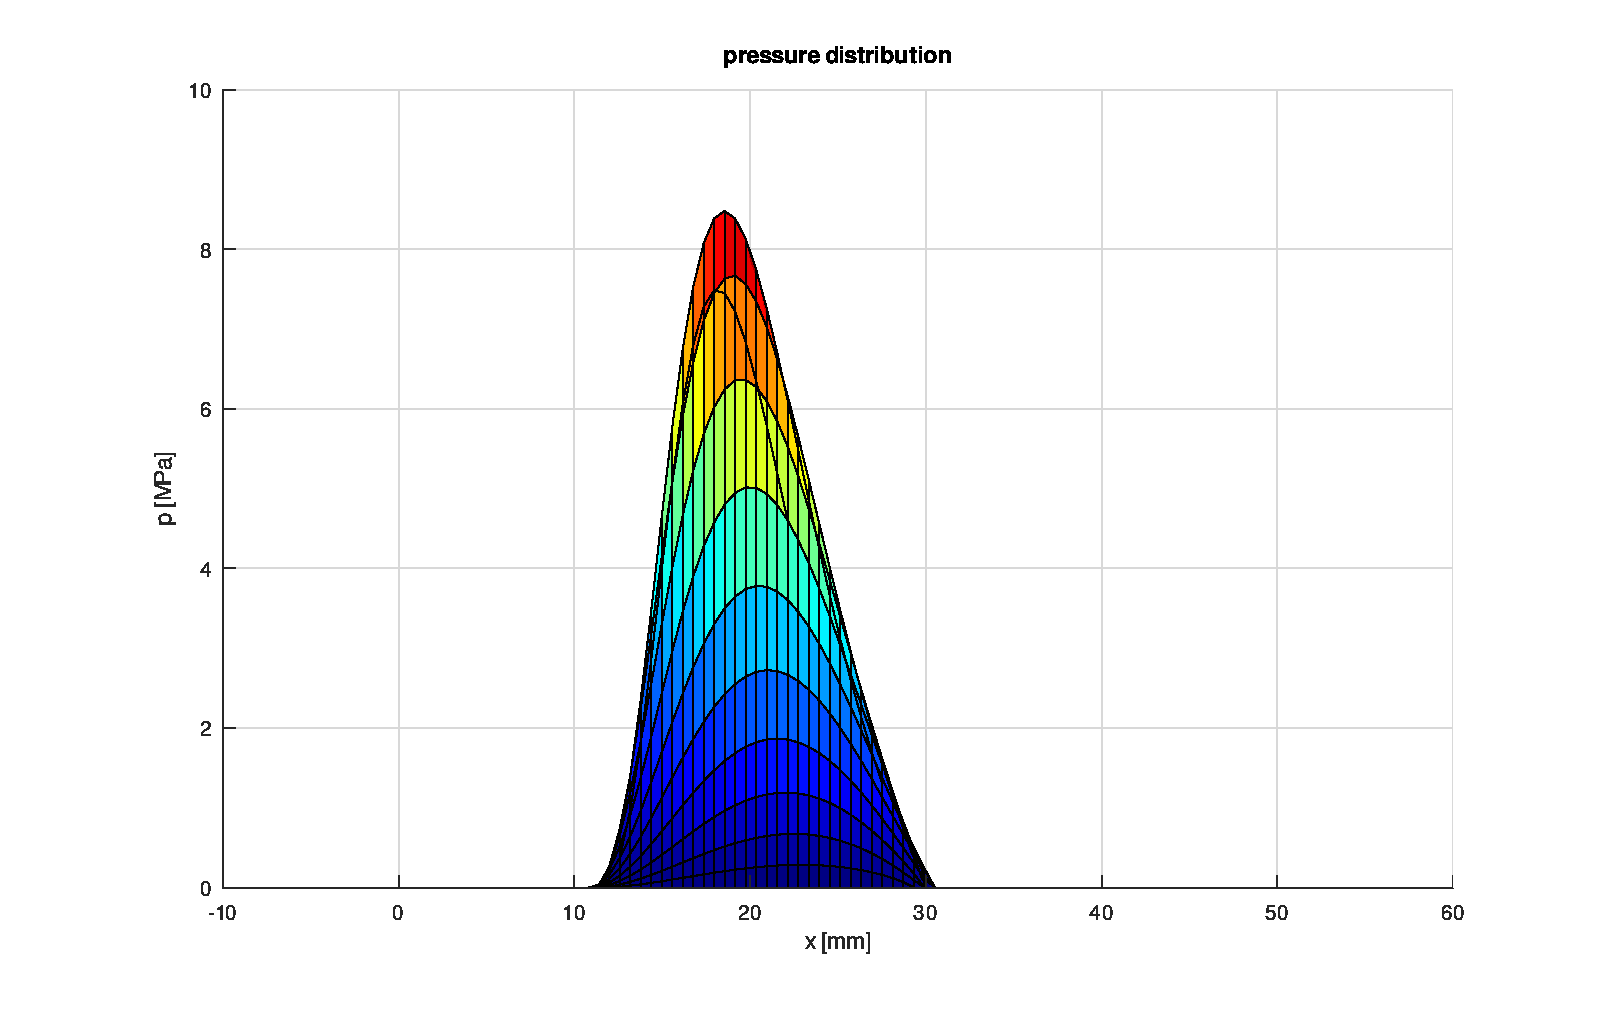
\includegraphics[width=\linewidth]{hydrodynamic_bearing}
\caption{Pressure distribution in the bearing}
\label{fig:hydrodynamic_bearing_pressure}
\end{figure}
